% !TEX root = ../main.tex
%

\section{Results}

\subsection{Main findings}

Figure \ref{fig::toxicity_aq_stats} shows the mean difference in toxicity and argument quality between each moderation strategy. Discussions where a moderator is absent feature overall significantly increased toxicity and decreased argument quality. Some strategies seem to have both statistically (Kruskal-Wallis $p=0$ for both measures) and qualitatively significant impact on discussions. Our proposed \ac{RL}-inspired strategy (see Section \ref{ssec:setup:strategies}) significantly outperforms all baselines, as well as all other established strategies, by a smaller margin. This is more evident when looking at toxicity. In fact, contrary to our expectations, the strategies based on widely used guidelines do not seem to outperform the baselines (apart from the moderator being absent).

\begin{figure*}[t]
    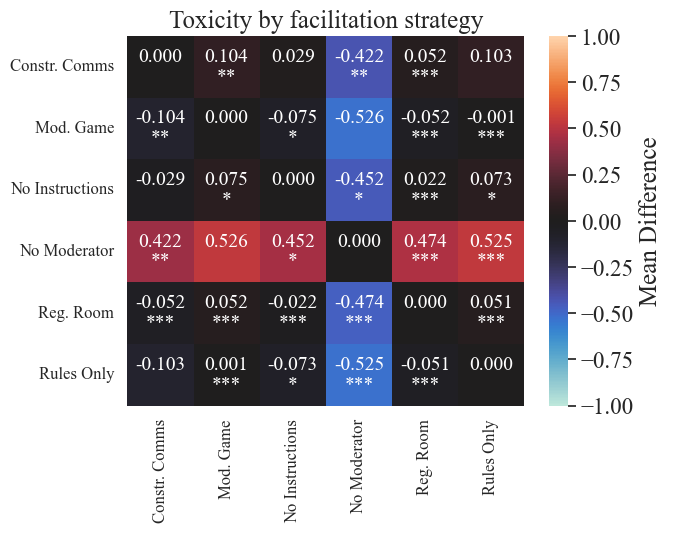
\includegraphics[width=0.48\linewidth]{toxicity_stats.png} \hfill
    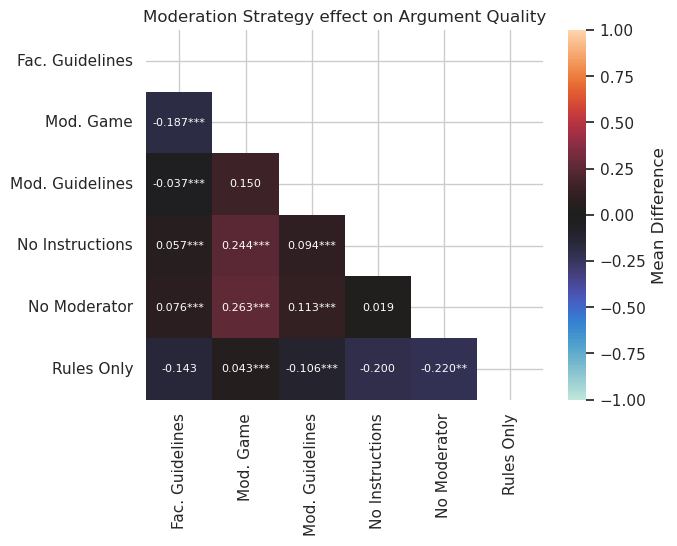
\includegraphics[width=0.48\linewidth]{argumentq_stats.png}
	\centering
	\caption{Mean difference of Toxicity (left) and Argument Quality (right) between each moderation strategy. $A[i, j] = 0.3^{***}$ indicates that the strategy $j$ is better than the strategy $i$ for an average of $0.3$ points with $p<0.001$. Each comparison is accompanied by Dunn's posthoc test for multiple comparisons \cite{dunn}, in the form of significance asterisks.}
	\label{fig::toxicity_aq_stats}
\end{figure*}


\subsection{Ablation study}

\subsubsection{Models}

Figure \ref{fig::discussion_variance} demonstrates that the Qwen-2.5 model features the largest amount of variance, while LLaMa-3.1 struggles the most to create diverse responses. Qwen-2.5 also produces relatively shorter comments, while LLaMa-3.1's are almost double the size on average (Addendum Figure \ref{fig::comment_length}). Contrary to expectations, the abliterated model does not produce more diverse, nor more toxic comments in average. This may indicate that models subjected to intense alignment procedures may not be able to replicate human behavior as authentically as other models (as reported in \citet{Park2023GenerativeAI}), although abliteration may not be an effective way of getting around alignment. 

\begin{figure}
	\centering
	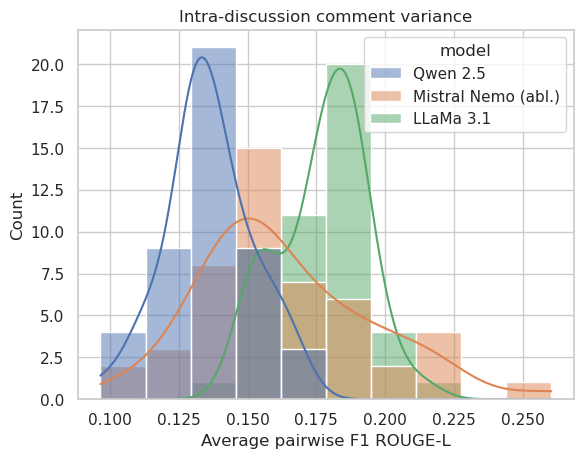
\includegraphics[width=\columnwidth]{discussion_variance.png}
	\caption{Histogram of the average pairwise F1 ROUGE-L scores (see Equation \ref{eq:variety}) for each discussion split by the \ac{LLM} that produced it.}
	\label{fig::discussion_variance}
\end{figure}


\subsection{Observations}

\subsubsection{LLM moderators}

As demonstrated by Figure \ref{fig::intervention_count}, \ac{LLM} moderators will respond at almost every point in the discussion. We also observe that \ac{LLM} user-agents are unusually lenient towards repeated, unneeded interventions of moderators, which is not representative of human behavior. In this situation, human users tend to get irritated, and we can usually observe a rise in toxicity \cite{schaffner_community_guidelines, make_reddit_great, proactive_moderation, cresci_pesonalized_interventions}.

